%%%%%%%%%%%%%%%%%%%%%%%%%%%%%%%%%%%%%%%%%%%%%%%%%%%%%%%%%%%%%%%%%%%%%%%%%%%%%%%
%% StuPro B, "Programmierumgebung Offener Antrieb" (POA)
%% Entwurf
%% $Id: entwurf.tex,v 1.4 2004/06/07 23:32:46 vanto Exp $
%%%%%%%%%%%%%%%%%%%%%%%%%%%%%%%%%%%%%%%%%%%%%%%%%%%%%%%%%%%%%%%%%%%%%%%%%%%%%%%
\documentclass[a4paper,titlepage,12pt,ngerman]{scrbook}
\usepackage{../common/header}
\usepackage{longtable}

\RCSdef $Revision: 1.4 $
\RCSdef $Date: 2004/06/07 23:32:46 $

\newcommand\version{Version \today \xspace}
%\newcommand\version{Version 1.0\xspace}

\title {\huge \product\\[0.5cm]\large Entwurf\\[0.5cm] \version
  \\[1cm] \Large \company}

\begin{document}

%%%%%%%%%%%%%%%%%%%%%%%%%%%%%%%%%%%%%%%%%%%%%%%%%%%%%%%%%%%%%%%%%%%%%%%%%%%%%%%
%% Deckblatt

\begin{titlepage}
\renewcommand{\thefootnote}{\fnsymbol{footnote}}
{\Huge
\raggedright
\textbf{POA} \\
\huge Programmierumgebung Offener Antrieb
\rule{\textwidth}{0.75pt}
\par
}
\begin{flushleft}
\normalsize
\version
\end{flushleft}
\vfill

{\parindent=0cm
\Huge Entwurf
}


\setcounter{footnote}{0}
\end{titlepage}

%%%%%%%%%%%%%%%%%%%%%%%%%%%%%%%%%%%%%%%%%%%%%%%%%%%%%%%%%%%%%%%%%%%%%%%%%%%%%%%
%% Versionsgeschichte

\section*{Versionsgeschichte}

\begin{itemize}

\item Version 1.0 (1.4.2003)

  Diese Version wurde dem Auftraggeber vorgelegt.

\end{itemize}

%%%%%%%%%%%%%%%%%%%%%%%%%%%%%%%%%%%%%%%%%%%%%%%%%%%%%%%%%%%%%%%%%%%%%%%%%%%%%%%
%% Inhaltsverzeichnis

\tableofcontents

%%%%%%%%%%%%%%%%%%%%%%%%%%%%%%%%%%%%%%%%%%%%%%%%%%%%%%%%%%%%%%%%%%%%%%%%%%%%%%%
%% Einleitung

%%%%%%%%%%%%%%%%%%%%%%%%%%%%%%%%%%%%%%%%%%%%%%%%%%%%%%%%%%%%%%%%%%%%%%%%%%%%%%%
%% StuPro B, "Programmierumgebung Offener Antrieb" (POA)
%% Projektplan
%% $Id: einleitung.tex,v 1.3 2003/06/07 16:01:04 garbeam Exp $
%% Achtung: Diese Datei wird ins Angebot inkludiert!
%%%%%%%%%%%%%%%%%%%%%%%%%%%%%%%%%%%%%%%%%%%%%%%%%%%%%%%%%%%%%%%%%%%%%%%%%%%%%%%

\chapter {Einleitung}
\section {Beschreibung des Projektplan}

Dieses Dokument ist Teil eines Angebotes �ber eine Projektdurchf�hrung
im Rahmen des Studienprojektes B ``Programmierumgebung Offener
Antrieb'' am ISW, Universit�t Stuttgart.

Der Projektplan gibt zu diesem Zeitpunkt eine grobe Einsch�tzung des
zu erwartenden Projektverlaufes wider. Der Plan wird w�hrend des
Projekts laufend angepasst.

\section {Entwicklungsphilosophie}

Das Projekt ist im wesentlichen durch zwei Bedingungen gepr�gt:\\

Auf der funktionalen Ebene sind die Anforderungen unscharf und
unterliegen st�ndigen �nderungen, da die Hardware, die von der zu
erstellenden Software programmiert werden soll, parallel dazu
entwickelt wird. Daraus ergeben sich auch w�hrend des Projektverlaufes 
neue Anforderungen.

Die zweite Einschr�nkung betrifft den zeitlichen Ablauf des Projekts. Bis
Mitte Oktober 2003 wird f�r eine Pr�sentation ein lauff�higer
Prototyp der Software ben�tigt.

Um diesen Bedingungen gerecht zu werden dient ein
Inkrementell-Iteratives Prozessmodell (siehe Balzert, Helmut: Lehrbuch
der Software-Technik, Band 2, Spektrum, 1998) zur Entwicklung. Im
wesentlichen wird zu Anfang des Projektes eine Anforderungsanalyse
durchgef�hrt und ein Prototyp erstellt. Dieser wird dann in
sogenannten Sprints verbessert bis der gew�nschte Zustand erreicht
ist.

%%% Local Variables: 
%%% TeX-master: "angebot"
%%% End: 
%%% vim:tw=79:


%%%%%%%%%%%%%%%%%%%%%%%%%%%%%%%%%%%%%%%%%%%%%%%%%%%%%%%%%%%%%%%%%%%%%%%%%%%%%%%
%% Design

%%%%%%%%%%%%%%%%%%%%%%%%%%%%%%%%%%%%%%%%%%%%%%%%%%%%%%%%%%%%%%%%%%%%%%%%%%%%%%%
%% StuPro B, "Programmierumgebung Offener Antrieb" (POA)
%% Entwurf
%% $Id: design.tex,v 1.18 2004/06/16 12:00:12 squig Exp $
%% Achtung: Diese Datei wird in den Entwurf inkludiert!
%%%%%%%%%%%%%%%%%%%%%%%%%%%%%%%%%%%%%%%%%%%%%%%%%%%%%%%%%%%%%%%%%%%%%%%%%%%%%%%

% classname
\newcommand\cn[1]{{\bf \texttt{#1}}}
% method
\newcommand\m[1]{\texttt{#1}}

\chapter{Architektur}

\section{�bersicht}

Die Architektur von POA gliedert sich in stark zusammenh�ngende
Module, die durch schmale Schnittstellen miteinander kommunizieren und
so eine geringe Kopplung aufweisen. So kann jedes dieser Module
einzeln an ge�nderte Anforderungen angepasst werden, wobei die
Interoperabilit�t erhalten bleibt.

Auf diese Weise wird die gr��tm�gliche Flexibilit�t f�r die
Weiterentwicklung und Wartung der Software sichergestellt. Aufgrund
des forschungsnahen Charakters des POA-Projekts wurde auf die
Flexibilit�t der Architektur besonderer Wert gelegt.

\begin{figure}[h!]
  \centering
  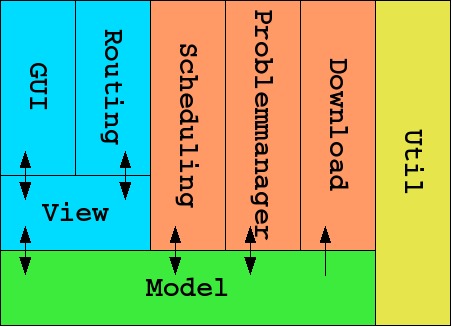
\includegraphics[width=10cm]{../abschlussbericht/design}
  \caption{POA Architektur}\label{arch_grafik}
\end{figure}

In Abbildung \ref{arch_grafik} werden die Module von POA
dargestellt. Im Folgenden wird eine kurze Beschreibung gegeben,
Details folgen im Kapitel \ref{modules}.

Die gr�n dargestellten Module bilden die Basis des
POA-Systems. Entw�rfe f�r Regler auf dem Offenen Antrieb werden in
Projekten (\ref{model}) entwickelt. Die Daten eines Projekts werden
in den Models des Projekts gespeichert.

Die rot dargestellten Module, Problemmanager (\ref{problem_manager}),
Scheduling (\ref{scheduling}) und Download (\ref{download}), bilden die
wesentlichen Aufgaben von POA ab.

\begin{itemize}
\item Pr�fen der Integrit�t eines Projekts und Anzeige der
  aufgefundenen Probleme
\item Automatische Berechnung eines optimalen Schedulings f�r das
  Netzwerk von Bl�cken
\item Compilation des Sourcecodes und Download auf die spezifizierten
  CPUs
\end{itemize}

Die in blau eingef�rbten Module realisieren die
Benutzungsschnittstelle von POA. Das Modul GUI umfasst Klassen zur
Darstellung von Dialogen. Die Views (\ref{view}) visualisieren die
relevanten Nutzdaten und das Routing-Modul (\ref{routing}) wird eingesetzt, um
Konnektoren �berkreuzungsarm in ein Netzwerk einzubringen.

Schlie�lich bietet das Utils Modul diverse Funktionalit�t, die h�uftig
ben�tigt wird. Die Klassen dieses Moduls sind Kandidaten um in
folgenden Projekten wiederverwendet zu werden.

\subsection{Projekte in POA}

Um mehrere Konfigurationen des Offenen Antriebs bearbeiten zu k�nnen,
stellt POA das Projekt-Konzept zur Verf�gung. Die Arbeit an einer
bestimmten Konfiguration (alle Bl�cke, Konnektoren, Source Code,
Layout der Darstellungen) wird in ein Projekt
zusammengefasst. Projekte k�nnen als ganzes auf st�ndigen Speicher
gespeichert und von diesem geladen werden.

Aufgrund ihrer zentralen Stellung bietet die Sicht auf ein Projekt
ebenfalls einen guten Ausgangspunkt f�r die Betrachtung der
Architektur. (siehe auch \ref{project})

\subsection{Speicherung von Projekten}

Projekte werden in einem Projekt-Ordner auf der Festplatte
gespeichert. Der Name des Ordners ist gleichzeitig der Name des
Projekts. Der Projekt-Ordner enth�lt die Datei project.xml, die alle
Projekt-Daten enth�lt.

Zus�tzlich gibt es f�r jede CPU des Projekts einen Unter-Ordner, der
die wiederum die Ordner inc f�r zu inkludierende
C-Pr�prozessor-Definitionen oder C-Deklarationen, lib f�r Bibliotheken
gegen die der selbstgeschriebene Code zu linken ist, und src f�r den
Quelltext f�r die CPU enth�lt. F�r diesen Quelltext kann POA
Rahmencode generieren.

\section{Module}
\label{modules}

Die Architektur von POA l�sst sich in stark zusammenh�ngende
Module aufteilen, die eine gerine Kopplung aufweisen. In den folgenden
Abschnitten sind diese Module im Detail beschrieben.

Die Zuordnung von einzelnen Klassen zu Modulen l�sst sich in der Regel
aus dem Klassennamen ableiten oder ist aus dem
Software-Architektur-Poster anhand der Schattierung ersichtlich.

\subsection{Datenmodell (Model)}
\label{model}

In den Model-Klassen wird das Datenmodell eines Projekts
repr�sentiert. In POA werden Daten in Objekten der Klassen
\cn{BlockModel} und \cn{PinModel}, sowie abgeleiteter Klassen
gespeichert. Die Klasse \cn{Projekt} verwaltet die Model-Objekte. Sie
dient als Container und stellt Methoden zur serialisierung und
deserialisierung von Projekten in einem POA spezifischen XML-Format
zur Verf�gung. Wird ein Projekt ver�ndert, d.h. ein Block hinzugef�gt,
entfernt oder ver�ndert, muss die Methode \m{setModified()}
aufgerufen werden.

\subsubsection{Serialisierung}

Der Mechanismus zum Erstellen des XML Dokuments bzw. des Datenmodells
aus einem XML Dokument ist in den Model-Klassen gekapselt. So ist es zum
Einen m�glich, jedes Objekt unabh�ngig vom Projekt zu serialisieren,
zum Anderen vereinfacht es die Wartbarkeit. Bei Erweiterungen der
Model-Klasse um weitere Datenfelder m�ssen nur die \m{serialize()} und
\m{deserialize()} Methoden angepasst werden, der Code in der Klasse \cn{Project}
bleibt gleich. Wichtig ist hier, dass bei abgeleiteten Klassen immer
die serialize/deserialize-Methoden der Superklasse aufgerufen werden,
da sich der Mechanismus auf die gesamte Klassenhierarchie verteilt. 

F�r die Erzeugung von Objektinstanzen bei der Deserialisierung ist die
Klasse \cn{ModelFactory} zust�ndig. Sie erzeugt anhand der
XML-Attributs ''block-type'' in dem jeweiligen XML-Element das
entsprechende Model-Objekt. �ber die Methoden \m{addBlock()} und
\m{removeBlock()} werden dem Projekt neue Modellbl�cke bekannt
gemacht bzw. wieder entfernt.

\subsubsection{Klassenhierarchie}

Die Model-Klassen sind von der abstrakten Klasse \cn{AbstractModel}
abgeleitet. Die Methode \m{createView(GridCanvas*)} erzeugt f�r
eine Model-Object eine korrespondierendes View-Object. Eine Aufruf der
Methode \m{updatePerformed()} benachrichtigt das View-Object �ber
�nderungen im Zustand des Model-Objects und sollte aufgerufen werden,
wenn z.B. die Taktraten eines Blocks ge�ndert wurde.

Die Klasse \cn{BlockModel} ist von \cn{AbstractModel} abgeleitet und
repr�sentiert Bl�cke mit Pins. Ausserdem werden in ihr Informationen
zum Laufzeitverhalten der Bl�cke abgelegt. �ber die Methoden
\m{addPin(PinModel*)} bzw. \m{deletePin(PinModel*)} wird dem Block ein
Pin hinzugef�gt bzw. wieder entfernt. Bei Aufruf der Methode
\m{addPin(PinModel*)}, erfolgt eine Benachrichtigung an das
korrespondierende View-Objekt �ber das Signal \m{pinAdded(PinModel*)}.
Wird ein \cn{BlockModel}-Objekt gel�scht wird das Signal
\m{deleted(BlockModel*)} gesendet, und das View-Objekt gel�scht.

Die n�chste Verfeinerung der Vererbungshierarchie erm�glicht die
Spezialisierung auf CPUs und Muxes, die es erm�glichen, Verbindungen
zwischen Bl�cken zu multiplexen. Ein CPU-Block (\cn{CpuModel}) erh�lt
die neuen Felder \m{autoRuntime}, \m{cpuId} und \m{source}.  Diese
Felder erm�glichen die automatische Laufzeitdauerberechnung, die
Erfassung der Id, die die CPU auf dem CPLD identifiziert sowie der
C-Quellcode der NIOS-CPU.  Ein Mux-Block (\cn{MuxModel}) verwaltet
einen Container mit \cn{MuxMapping}-Objekten. In diesen wird das
Mapping von Pins auf Pins mit unterschiedlichen Bitbreiten erm�glicht.

Instanzen der Klasse \cn{PinModel} repr�sentieren die einzelnen Pins
eines Blocks. Wenn eine Verbindung zwischen zwei Bl�cken hergestellt
wird, so m�ssen auch die Pins �ber dar�ber benachrichtigt werden. Das
geschieht �ber einen Aufruf der Methode \m{attach(PinModel*
  connectTo)}. Wurde eine Verbindung erstellt, gibt die Methode
\m{connected()} gibt den Pin des anderen Blocks zur�ck. Ausserdem
haben Pins einen Namen (\m{name}), eine Adresse (\m{address}), eine
Bitbreite (\m{bits}), eine Id (\m{id}), sowie eine Position
(\m{position}), die die Reihenfolge der Pins wiederspiegelt. Der Typ
eines Pins kann die Werte \m{PinType::INPUT}, \m{PinType::OUTPUT} und
\m{PinType::EPISODIC} annehmen. �ber den Konstruktor wird dem Pin der
Vaterblock mitgeteilt. Dieser kann �ber \m{parent()} abgefragt werden.
Die Signale \m{deleted(), detached()} und \m{updated()} benachtigten
interessierte Klassen, wenn ein Pin entfernt werden soll, wenn eine
Verbindung gel�st wurde oder wenn Eigenschaften des Pins ver�ndert
wurden. In der derzeitige Implementierung h�ren nur die
\cn{BlockView}-Instanzen auf diese Signale.

\subsubsection{Drag and Drop}

Zum visuellen erzeugen von Bl�cken wird bei POA die Drag\&Drop-Idee
verwendet. Dazu zieht der Benutzer ein Objekt aus der Blockbibliothek
in den Arbeitsbereich (\cn{GridCanvas}). Unter der
Haube werden die Objekte beim Herausziehen aus der Bibliothek �ber die
Serialisierungsmethoden in einen XML-String umgewandelt und beim
''fallen lassen'' �ber die \cn{ModelFactory} instanziert, von
Bibliotheksinformationen bereinigt und in das Projekt eingef�gt. Das
dazugeh�rige View-Objekt wird an den aktuellen Maus-Koordinaten
erstellt.  Das Einf�gen in die Bibliothek funktioniert analog dazu.
Die Zwischenablagefuntionen sind genauso implementiert. Beim Kopieren
eines Objekts werden die Daten serialisiert und in die Zwischenablage
kopiert und beim Einf�gen wieder deserialisiert. Da z.B. bei CPUs der
Sourcecode mitkopiert werden soll, ist f�r die
Copy\&Paste-Funktionalit�t eine erweiterte Serialisierung notwendig.
Daher sieht die abstrakte Superklasse f�r die Serialisierung f�r die
Zwischenablage eine eigene Methode vor: \m{serializeCopy()}.

\subsection{View}
\label{view}

Views werden verwendet, um dem Benutzer die Daten zu pr�sentieren. Sie
werden �ber Signals benachrichtigt, wenn sich ein Model ver�ndert und
passen dann die grafische Darstellung entsprechend an.

Der \cn{GridCanvas} ist eine Arbeitsoberfl�che f�r ein POA-Netzwerk. Die
Basisklasse f�r den \cn{GridCanvas} sowie f�r alle Views darauf werden von
der QT-Bibliothek gestellt. F�r POA musste nur eine Spezialisierung
dieser Basisfunktionalit�t durchgef�hrt werden.

Die \cn{GridCanvas}-Objecte werden in der \cn{Project}-Klasse
verwaltet. Zu jedem Projekt kann es mehrere \cn{GridCanvas}-Instanzen
geben. Diese Funktionalit�t wird bisher allerdings nicht genutzt, es
wird immer nur ein \cn{GridCanvas} pro Projekt angezeigt.

Ohne selbst als Model gelten zu k�nnen, stellt der \cn{GridCanvas} nur eine
virtuelle Arbeitsoberfl�che dar. F�r die Darstellung eines Teils des
\cn{GridCanvas} sind \cn{CanvasView}-Objekte zust�ndig. So kann dieselbe
Arbeitsoberfl�che in mehreren Fenstern ge�ffnet werden und in jedem
Fenster kann ein anderer Ausschnitt der Arbeitsoberfl�che angezeit
werden.

Die meisten Views, die speziell f�r POA entwickelt wurden, repr�sentieren
grafische Objekte auf einem \cn{GridCanvas}. Dazu geh�ren \cn{BlockView},
\cn{PinView} und \cn{TextView}.

Eine besondere Behandlung ist allerdings f�r Konnektoren notwendig.
Konnektoren k�nnen auf dem Canvas nicht ohne weiteres dargestellt
werden, weil Qt seine Funktionalit�t hier auf wenige geometrische
Objekte beschr�nkt. Die Linienz�ge die In POA verwendet werden,
bestehen deshalb aus mehreren \cn{ConnectorViewSegment}-Objekten. Um
von der Verwaltung der einzelnen Segmente zu abstrahieren wurde die
Klasse \cn{ConnectorViewList} eingef�hrt. Objekte dieser Klasse
agieren als View f�r ein Verbindung zwischen zwei
\cn{PinModel}-Objekten, aber delegieren die tats�chliche
Darstellungsaufgabe an mehrere \cn{ConnectorViewSegment}-Objekte.

\subsection{Controller}
\label{controller}

Als Controller wird die Komponente bezeichnet, die Benutzereingaben
und interne Ereignisse verarbeitet und die Synchronisation zwischen
View und Model sicherstellt.

Aktionen, die der Benutzer durch Eingaben anst��t, l�sen in QT Signals
aus. Diese Signals werden in POA lokal in dem entsprechenden
View-Objekt verarbeitet, z.B. in \cn{CanvasView} f�r alle Aktionen,
die auf dem Canvas geschehen (z.B. Selektieren eines Blocks) oder in
MainWindow (z.B. bei Aktivieren eines Men�punkts). Aufw�ndige
Bearbeitungen werden in spezielle von der Klasse \cn{CanvasViewAction}
abgeleitete Objekte ausgelagert.

Eine besondere Auslagerung der Controller bietet sich f�r POA nicht
an. Die Benutzer-Eingaben erfolgen auf einer bestimmten View und das
zugeh�rige View-Objekt hat die n�tigen Kompetenzen, um die Eingabe zu
verarbeiten. Falls eine Bearbeitung mehrere Schritte erfordert, so
erzeugt das View-Objekt ein Action-Objekt, um die Aufgabe zu
erledigen.

\subsection{Scheduling}
\label{scheduling}

Optimales Scheduling bedeutet in POA die Berechnung eines optimalen
Offsets f�r jeden Block, da die Taktraten f�r jeden Block bereits
feststehen.

Die optimalen Offsets werden in POA f�r bestimmte Signalpfade
berechnet. Hierzu dient dienen Objekte der Klasse Path. F�r jeden
gew�nschten Signallaufpfad wird ein solches Objekt erzeugt. Dann kann
die Signallaufzeit minimiert werden, indem alle Path-Objekte in einer
definierten Reihenfolge einzeln optimiert werden.

Die Path-Objekte verwenden dazu eine Graph-Struktur, die von der
Klasse \cn{BlockGraph} angeboten wird. Ein \cn{BlockGraph} besteht aus
einer Reihe von \cn{BlockNode}-Objekten. In den
\cn{BlockNode}-Objekten kann ein Flag gesetzt werden. Anhand dieses
Flags erkennt der Optimierungsalgorithmus, ob ein bestimmter Knoten
bereits einen optimalen Offset erhalten hat, oder noch ver�ndert
werden darf.

Eine Auswahl von Signallaufpfaden, kann der Benutzer in dem
AutoSchedulingDialog vornehmen. Dieser Dialog bedient sich des
BlockGraphs, um eine Liste aller Bl�cke anzuzeigen, die noch in keinem
Pfad enthalten sind.

\subsection{Download}
\label{download}

Der Download ist in der Klasse \cn{DownloadManager} implementiert. Zur
�bertragung der Daten wird die QExtSerialPort-Bibliothek verwendet.
Die Bibliothek einheitliche Methoden zum Zugriff auf die serielle
Schnittstelle f�r Windows und Linux. Die Initialisierung erfolgt in
der \m{initializeAndOpen()} Methode. Hier k�nnen die fest
programmierten �bertragungsparameter und die Geschwindigkeit ge�ndert
werden. Die �bertragung der Daten erfolgt in der \m{download()}
Methode und kann hier angepasst werden, falls sich das
�bertragungsprotokoll �ndert. In der aktuellen Implementierung kann
der kompilierte Quellcode einer einzelnen CPU �bertragen werden.
 
\subsection{Routing}
\label{routing}

Die Routing Schnittstelle ist sehr abstrakt definiert. Es wird
lediglich die Verbindung zweier Punkte auf einem GridCanvas gefordert.
Zwei Routing Algorithmen mit sehr unterschiedlichen Eigenschaften
implementieren diese Schnittstelle.

Der \cn{DirectRouter} stellt die Verbindung anhand von Fallunterscheidungen
mit der geringsten Anzahl von Knickpunkten her ohne �berschneidungen
zu ber�cksichtigen. Der Algorithmus ist ausreichend schnell, um die
Verbindungen w�hrend des Verschiebens von Bl�cken simultan
neuzuberechnen. 

Der \cn{DijkstraRouter} benutzt den Dijkstra Algorithmus um eine optimale
Route mit m�glichst wenig Knickpunkten und �berschneidungen zu finden.
Auf Grund der Vielzahl der m�glichen Wege betr�gt die Laufzeit des
Algorithmus in der Regel ein vielfaches des DirectRouter.

Durch Ableitung der \cn{ConnectorRouter} Klasse und Erweiterung der
\cn{GridCanvas} Klasse ist eine Implementierung von zus�tzlichen
Routing-Algorithmen m�glich.

\subsection{Problemmanager}
\label{problem_manager}

Die Klasse \cn{ProblemReportManager} validiert ein Projekt und stellt
eine Baumansicht mit den Ergebnissen zur Verf�gung. Im ersten Schritt
werden alle Bl�cke sequentiell gepr�ft. Im zweiten Schritt werden die
Verbindungen zwischen den Bl�cken gepr�ft. Die Validierung erfolgt in
der \m{report()}-Methode und \m{checkBlock()}-Methode. Hier k�nnen
weitere Pr�fungen eingef�gt werden. F�r jeden Fehler wird ein Objekt
vom Typ \cn{ProblemReportItem} erzeugt, das in dem Ergebnissbaum
angezeigt wird.

\subsection{Querschnittsmodule}

Einige Klassen k�nnen keinem Modul zugeordnet werden, da diese von
vielen Modulen benutzt werden. Einige dieser Querschnittsklassen sind
im folgenden beschrieben.

\subsubsection{Einstellungen (Settings)}

In der \cn{Setting}-Klasse werden globale Einstellungen wie Farben, Schriftarten
und Pfade verwaltet, die zum Teil auch �ber den Einstellungsdialog vom
Benutzer ge�ndert werden k�nnen. �nderungen von Einstellungen, die
direkt in der Anwendung sichtbar gemacht werden sollen, werden �ber
entsprechende Signale bekannt gemacht.


%%% Local Variables: 
%%% TeX-master: "entwurf"
%%% End: 
%%% vim:tw=79:


\section{Persistenz}

\subsection{XML Format}
Die POA-Datenmodelle werden im XML-Format im Projektverzeichnis abgelegt.

Die Datei gliedert sich auf h�chster Ebene in zwei Teile, die von dem
Wurzelelement umschlossen werden. Der erste Teile repr�sentiert das
Datenmodell, der zweite Teil bezieht sich auf die Darstellung der
Bl�cke. Diese View-Elemente beziehen sich �ber eine ID auf den
jeweiligen Block im Modell-Bereich. Eine Ausnahme bilden hier die
Verbindungen zwischen Bl�cken. Diese haben keine Modellinstanz sondern
werden nur als View-Element abgespeichert.

Die folgende Abbildung verdeutlicht den Aufbau der Projektdatei.

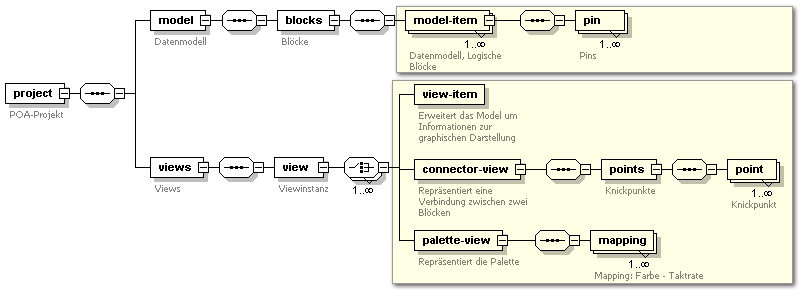
\includegraphics[width=17cm]{poa-schema.png}

\subsubsection{Struktur}
Die Projektdatei wird durch die folgenden Elemente strukturiert.

\begin{longtable}[c]{|p{5.466cm}|p{5.466cm}|p{5.466cm}|}
\hline
{\bf Element} & {\bf Unterelemente} & {\bf Beschreibung}\\\hline
\endhead
project      & model, view  & Wurzelelement \\\hline
model        & blocks       & Leitet den Modellbereich ein\\\hline
blocks       & model{}-item & Enth\"alt die Blockbeschreibungen\\\hline
model{}-item & pin          & Repr\"asentiert einen Block\\\hline
pin          &              & Repr\"asentiert einen Pin\\\hline
views        & view         & Leitet den Viewbereich ein\\\hline
view         & view{}-item, connector{}-view, palette{}-view &
Erweitert das Datenmodell um Darstellungsinformationen \\\hline

view{}-item  &              & Beschreibt die Position eines Blocks\\\hline
connector{}-view & points   & Beschreibt eine Verbindungslinie
zwischen zwei Bl\"ocken\\\hline

points & point & Enth\"alt die Knickpunkte der Verbindung\\\hline
point & & Repr\"asentiert einen Knickpunkt\\\hline
palette{}-view & mapping & Beschreibt die Position und die Eintr\"age
der Farbpalette \\\hline

mapping & & Verkn\"upft eine Taktfrequenz mit einer Farbe\\\hline
\end{longtable}


\subsubsection{Daten}
Die Projektdaten befinden sich in den Attributen der oben genannten Elemente.
\begin{longtable}[c]{|p{2.809cm}p{4.9420004cm}p{3.46cm}p{4.986cm}}
\hline
\multicolumn{1}{|p{2.809cm}|}{{\bf Element}} &
\multicolumn{1}{p{4.9420004cm}|}{{\bf Attribut}} &
\multicolumn{1}{p{3.46cm}|}{{\bf Datentyp}} &
\multicolumn{1}{p{4.986cm}|}{{\bf Beschreibung}}\\\hline
\endhead
model{}-item
&
\multicolumn{3}{p{13.788cm}}{\hspace*{-\tabcolsep}\begin{tabular}{|p{4.9420004cm}|p{3.46cm}|p{4.986cm}|}
id & int & Eindeutige Identifikation des Blocks\\\hline
name & String & Bezeichnung des Blocks\\\hline
desc & String & Beschreibung des Blocks in der Blockbibliothek\\\hline
hasOutputPins & boolean & Zeigt an, ob der Block Ausgangspins besitzt\\\hline
hasInputPins  & boolean & Zeigt an, ob der Block Eingangspins besitzt.\\\hline
hasEpisodicPins & boolean & Zeigt an, ob der Block episodische Pins
besitzt.\\\hline

clock & int & Taktrate des Blocks (ns)\\\hline
type  & String & Name der Rubrik unter der der Block in der
Blockbibliothek erscheint\\\hline
offset & int & Zeitlicher Versatz (ns)\\\hline
auto{}-offset & boolean & Zeigt an, ob der Versatz automatisch
berechnet wird\\\hline 

hasRuntime & boolean & Zeigt an, ob der Block eine Laufzeit besitzt.\\\hline
runtime & int & Laufzeit des Blocks (ns)\\\hline
block{}-type & \ {\quotedblbase}block``, {\quotedblbase}cpu`` &
Definiert den Typ des Blocks. {\quotedblbase}block`` repr\"asentiert
einen Core, {\quotedblbase}cpu`` eine CPU \\\hline
cpuid & int & Nummer der CPU auf dem CPLD \\\hline
\end{tabular}%\hspace*{-\tabcolsep}

}\\\cline{1-1}

pin&
\multicolumn{3}{p{13.788cm}}{\hspace*{-\tabcolsep}\begin{tabular}{|p{4.9420004cm}|p{3.46cm}|p{4.986cm}|}

id & int & Eindeutige Identifikation des Pins\\\hline
name & String & Bezeichnung des Pins\\\hline
address & int & Speicheradresse des Pins auf dem CPLD\\\hline
bits & int & Bitbreite des Pins\\\hline
type & {\quotedblbase}input``, {\quotedblbase}output``,
{\quotedblbase}episodic`` & Definiert um welche Art von Pin es sich
handelt\\\hline

position & int & Bestimmt die Reihenfolge der Pins am Block\\\hline
\end{tabular}\hspace*{-\tabcolsep}
}\\\cline{1-1}
\multicolumn{1}{|p{2.809cm}|}{
view

}&
\multicolumn{1}{p{4.9420004cm}|}{
name

}&
\multicolumn{1}{p{3.46cm}|}{
String

}&
\multicolumn{1}{p{4.986cm}|}{
Reserviert


}\\\hline

view{}-item


&
\multicolumn{3}{p{13.788cm}}{\hspace*{-\tabcolsep}\begin{tabular}{|p{4.9420004cm}|p{3.46cm}|p{4.986cm}|}


x, y & int & Position des Blocks auf dem Arbeitsbereich\\\hline
model{}-id & int & ID des {\textless}model{\textgreater}{}-Elements\\\hline
\end{tabular}\hspace*{-\tabcolsep}
}\\\cline{1-1}

connector{}-view


&
\multicolumn{3}{p{13.788cm}}{\hspace*{-\tabcolsep}\begin{tabular}{|p{4.9420004cm}|p{3.46cm}|p{4.986cm}|}


source{}-block, source{}-pin & int & Bestimmt Quell{}-Block und {}-Pin
f\"ur die Verbindung \"uber die jeweiligen Ids aus den
{\textless}model{\textgreater}{}-Elementen\\\hline

target{}-block, target{}-pin & int & Bestimmt Ziel{}-Block und {}-Pin
f\"ur die Verbindung \"uber die jeweiligen Ids aus den
{\textless}model{\textgreater}{}-Elementen\\\hline
\end{tabular}\hspace*{-\tabcolsep}
}\\\cline{1-1}
\multicolumn{1}{|p{2.809cm}|}{
point


}&
\multicolumn{1}{p{4.9420004cm}|}{
x, y


}&
\multicolumn{1}{p{3.46cm}|}{
int


}&
\multicolumn{1}{p{4.986cm}|}{
Position des Knickpunkts auf dem Arbeitsbereich


}\\\hline

palette{}-view


&
\multicolumn{3}{p{13.788cm}}{\hspace*{-\tabcolsep}\begin{tabular}{|p{4.9420004cm}|p{3.46cm}|p{4.986cm}|}


x, y & int & Position der Palette auf dem Arbeitsbereich\\\hline
last{}-pal{}-entry & int & Definiert die Index{}-Nummer auf der
Farbpalette, die f\"ur die n\"achste Taktrate verwendet werden soll\\\hline

name & String & Bezeichner der Palette (reserviert)\\\hline
\end{tabular}\hspace*{-\tabcolsep}
}\\\cline{1-1}

mapping &
\multicolumn{3}{p{13.788cm}}{\hspace*{-\tabcolsep}\begin{tabular}{|p{4.9420004cm}|p{3.46cm}|p{4.986cm}|}

ns & int & Taktfrequenz in Nanosekunden.\\\hline

pal{}-entry & int & Index{}-Nummer auf der Farbpalette.\\\hline
\end{tabular}\hspace*{-\tabcolsep}
}\\\cline{1-1}
\end{longtable}

\subsection{Document Type Definition}
%\lstset{% general command to set parameter(s)
%basicstyle=\small\sffamily, % print whole listing small
%keywordstyle=\color{black}\bfseries\underbar,
% underlined bold black keywords
%identifierstyle=, % nothing happens
%commentstyle=\color{white}, % white comments
%stringstyle=\ttfamily, % typewriter type for strings
%showstringspaces=false, % no special string spaces
%language=XML}

\lstset{
  language=XML, %The programminglanguage to be used
  basicstyle=\scriptsize\ttfamily, %The text size of the code
  keywordstyle=\color{red}\bfseries,
  stringstyle=\underbar,
  commentstyle=\color{blue}, % blue comments
  showspaces=false, %Leaves spaces blank
  showstringspaces=false, %Leaves spaces in strings blank
  breaklines=true, %Break lines that are too long
  fontadjust=true,
  extendedchars=false, %Includes danish charactors
  numbers = left, %Shows linenumbers
  stepnumber = 1 %The interval with which linenumbers are displayed
}
\begin{lstlisting}{language=XML}
<?xml version="1.0" encoding="UTF-8"?>
<!-- root element -->
<!ELEMENT project (model, views)>

<!-- model elements -->
<!ELEMENT model (blocks)>
<!ELEMENT blocks (model-item+)>
<!ELEMENT model-item (pin+)>
<!ATTLIST model-item
	offset CDATA #REQUIRED
	desc CDATA #REQUIRED
	hasOutputPins CDATA #REQUIRED
	hasInputPins CDATA #REQUIRED
	clock CDATA #REQUIRED
	runtime CDATA #REQUIRED
	hasEpisodicPins CDATA #REQUIRED
	type CDATA #REQUIRED
	id CDATA #REQUIRED
	name CDATA #REQUIRED
	auto-offset CDATA #REQUIRED
	hasRuntime CDATA #REQUIRED
	block-type (block | cpu) #REQUIRED
	cpuid CDATA #IMPLIED
	auto-runtime CDATA #IMPLIED
>
<!ELEMENT pin EMPTY>
<!ATTLIST pin
	address CDATA #REQUIRED
	bits CDATA #REQUIRED
	position CDATA #REQUIRED
	type (input | output | episodic) #REQUIRED
	id CDATA #REQUIRED
	name CDATA #REQUIRED
>

<!-- view elements -->
<!ELEMENT views (view)>
<!ELEMENT view (view-item | connector-view | palette-view)+>
<!ATTLIST view
	name CDATA #REQUIRED
>
<!ELEMENT view-item EMPTY>
<!ATTLIST view-item
	x CDATA #REQUIRED
	y CDATA #REQUIRED
	model-id CDATA #REQUIRED
>

<!-- connectors -->
<!ELEMENT connector-view (points)>
<!ATTLIST connector-view
	target-pin CDATA #REQUIRED
	target-block CDATA #REQUIRED
	source-pin CDATA #REQUIRED
	source-block CDATA #REQUIRED
>
<!ELEMENT points (point+)>
<!ELEMENT point EMPTY>
<!ATTLIST point
	x CDATA #REQUIRED
	y CDATA #REQUIRED
>

<!-- palette -->
<!ELEMENT palette-view (mapping+)>
<!ATTLIST palette-view
	last-pal-entry CDATA #REQUIRED
	x CDATA #REQUIRED
	y CDATA #REQUIRED
	name CDATA #REQUIRED
>
<!ELEMENT mapping EMPTY>
<!ATTLIST mapping
	ns CDATA #REQUIRED
	pal-entry CDATA #REQUIRED
>
\end{lstlisting}
%%%%%%%%%%%%%%%%%%%%%%%%%%%%%%%%%%%%%%%%%%%%%%%%%%%%%%%%%%%%%%%%%%%%%%%%%%%%%%%
%% Anhang

\appendix

\end{document}
%%% vim:tw=79:
